\chapter{Implementation}
\label{chap:implem}
\section {Development Environment Overview}
Incremental recogniser is implemented in Java programming language, using
an open-source project \textit {Incremental Spoken Dialogue processing
Toolkit} (InproTK), developed by the Universities of Potsdam, Bielefeld and
Hamburg. InproTK includes modules for speech recognition, speech understanding,
speech processing and dialogue management. Speech recognition module is based on
implemented Java Sphinx-4 recogniser, a package of CMU Sphinx speech recognition
toolkit.
\section {IU Modules and Data Processing}
\textit {Incremental Units} (IUs) are minimal information units in InptoTK.
IUs varies in the level abstraction (from low to high) and capable of
describing diverse types of information (phonemes, words, phrases, ...). IUs
of different abstraction levels form a IU network. An example of IU hierarchy is
shown in the figure.
\begin{figure}[htbp]
  \centering
    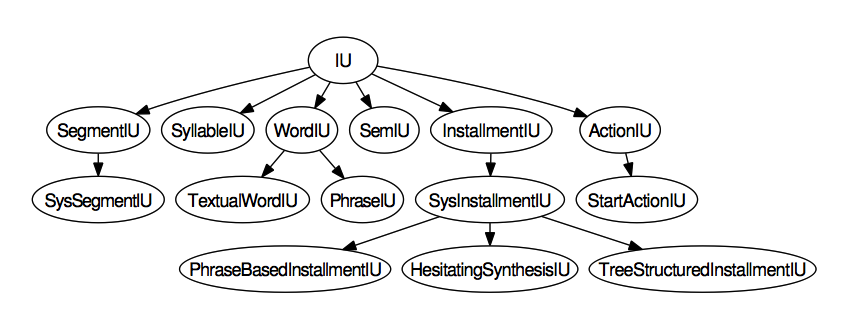
\includegraphics[width=1.0\textwidth]{images/IUs.png}
 \caption{ An excerpt of INproTk built-in type hierarchy \parencite
 {baumann2013:phd}.}
  \label{fig:IUs}
\end {figure}
Processing of IUs is guarantied by IU modules. IU
modules consist of left buffer, right buffer and processors.  
Different IUs modules are interconnected with each other, forming a pipeline of IU modules \parencite {baumann2013:phd}. A typical
communication between two IU modules is shown in the figure \ref{fig:IUs}.
\begin{figure}[htbp]
  \centering
    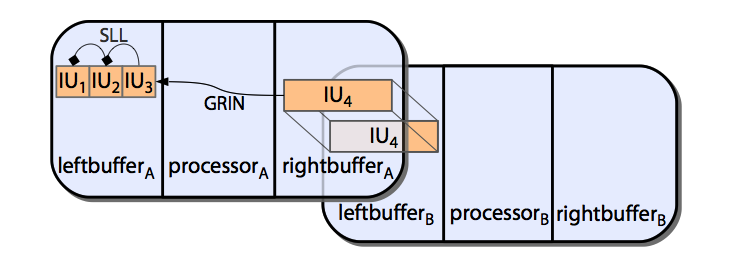
\includegraphics[width=1.0\textwidth]{images/iuandbuffer.png}
 \caption{ Incremental Modules and their intercommunication via left-right
 buffers \parencite {baumann2013:phd}.}
  \label{fig:IUs}
\end {figure}
\section {INproTK IU Modules in Google+Sphinx Recognizer Architecture}
\subsection  {Google IU Module}
GoogleASR is a source IU module in InproTK, which listens to the
results coming from Google's  downstream connection in JavaScript Object
Notation (JSON) format (see figure \ref{fig:json_ouput}) and passes results to
its listeners by updating the current hypotheses and providing information about the hypotheses time (hypotheses start and end times).

\begin{figure}[htbp]
  \centering
   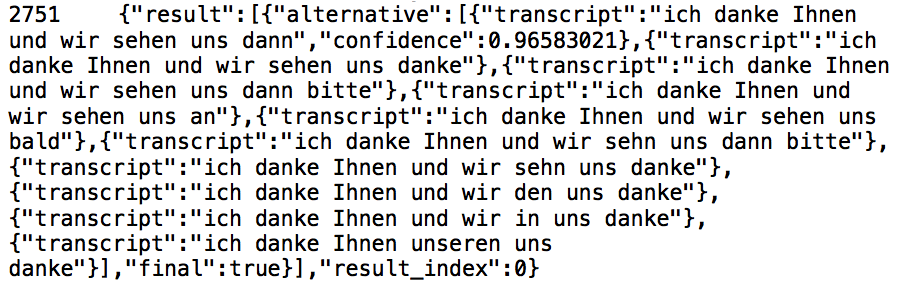
\includegraphics[width=1\textwidth]{images/json_extr.png}
    \caption{JSON file example}
      \label{fig:json_ouput}
\end{figure}

 Timing, implemented in Google ASR, has nothing to do with true alignment.
With the help of this information  it is only possible to calculate the
timeliness: FO as well as FD.  Manual reconstruction of alignment from
timeliness is problematic as timeliness does not preserve any information about word
duration. 

For example, in the figure  \ref {fig:google_ouput} the first hypothesis (word
\textit {ich}) equals 0 and end times equals about 7.5 time slots, whereas the
borders of the word \textit {ich} are between 1 and 3.5 time slot. In addition,
in case of Google we are dealing with additional output delay, resulted from network latency, which can be slightly variable approximately
between 10 and 200 ms depending on the network configuration. Google has
processed the file till the end of the word \textit {ich} by the time 3.5,
after some internal Google offset, the output was made.
It is assumed, that Google offset reflects the problem of stability of the
the output and latency \parencite {mcgrawgrauenstein2012}. Finally, Google ASR returned this result after 
a network delay.  
\begin{figure}[htbp]
  \centering
   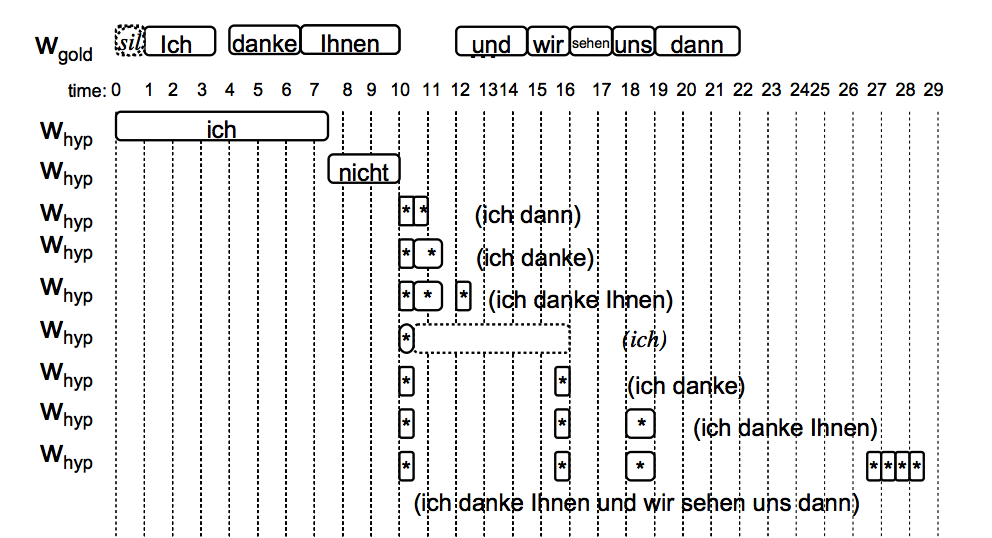
\includegraphics[width=0.9\textwidth]{images/google_output.png}
  \caption{Incremental output of Google ASR with existing timing.}
  \label{fig:google_ouput}
\end{figure}

 
\subsection {Sphinx ASR Module and Label Writer in INproTK}
Sphinx ASR in INproTk is a module that receives results from Sphinx-4
recognizer, transforms them to IUs of recognized words and sends them
to label writer.   Label writer in its turn
is responsible for output of the recognition results and  their timing
information in the console. Apart from that label writer  offers a configurable
option to save the recognition and timing results to a file. An extract of such
files can be found in the appendix \ref{chap:appB}. 

\section {Architecture Overview of the Google+Sphinx Recognizer}
Sphinx-Google architecture includes Sphinx-4 frontend, dictionary,
language model and acoustic model, decoder with search graph, forced alignment
module, Sphinx control thread, synchronous blocking queue and InproTK IUs:
Google ASR, Sphinx ASR and label writer (see figure \ref {fig:arch}).
\begin{figure}[htbp]
  \centering
    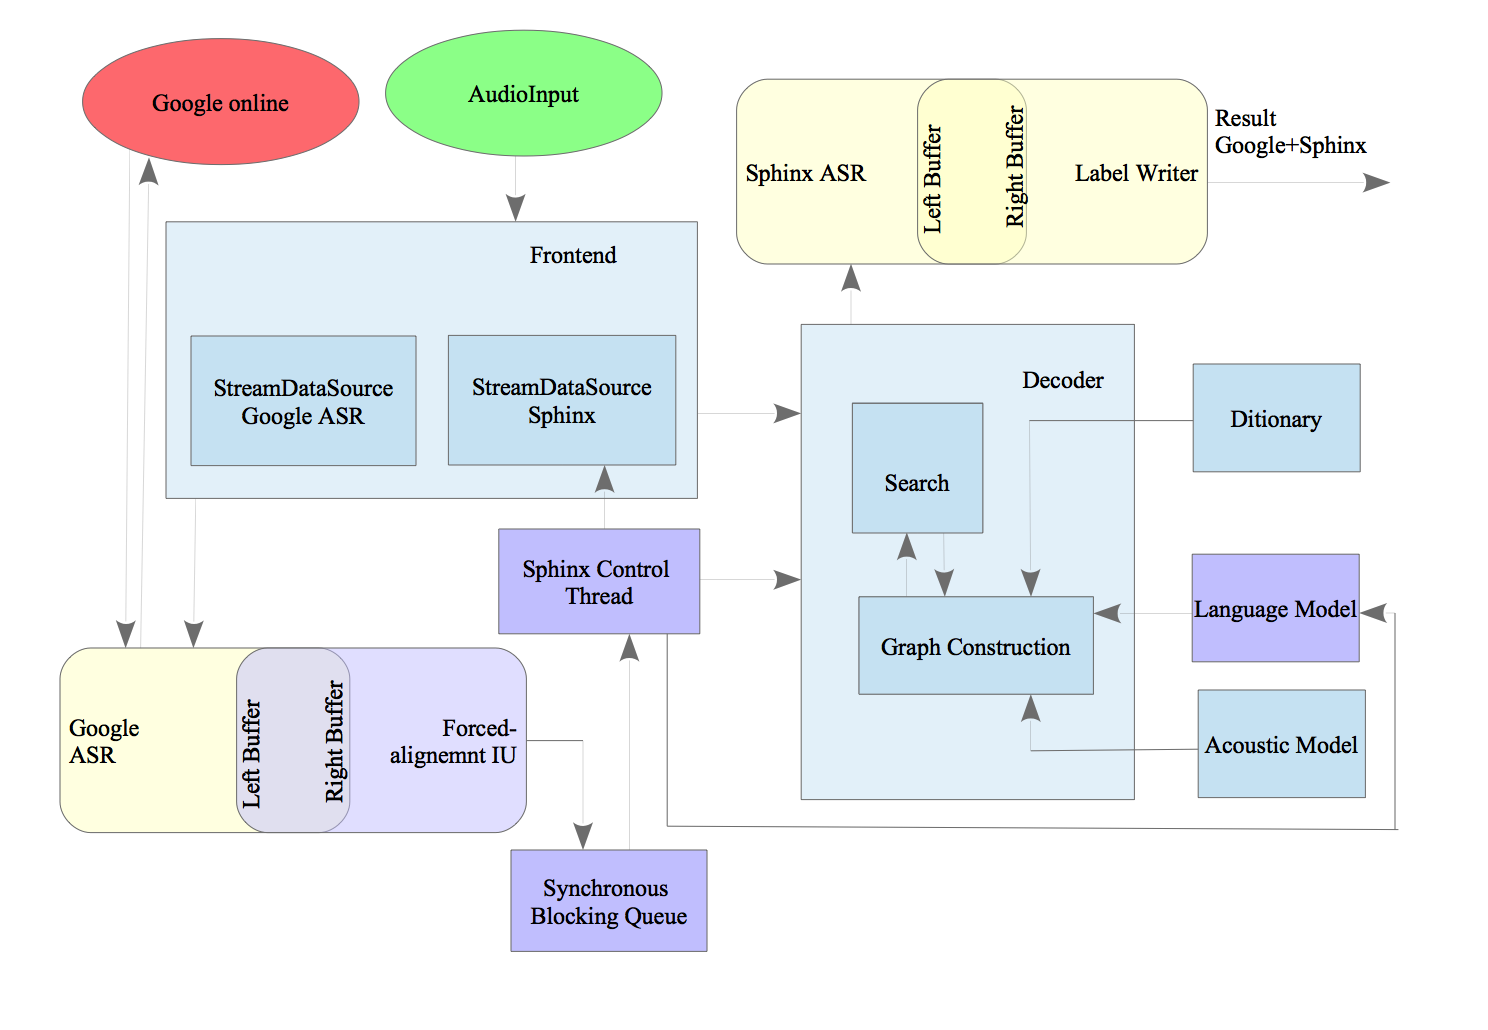
\includegraphics[width=1\textwidth]{images/architecture.png}
 \caption{Implementation Overview.}
  \label{fig:arch}
\end {figure} 
%\subsection {Frontend}

As an audio input both Google ASR and Sphinx receive the same audio input.
Input stream of Google ASR is set only once, whereas the length of
the stream is equal to the whole audio. By contrast, the Sphinx input stream is
updated every time Google ASR returns a new hypothesis.  


GoogleASR listens to JSON results coming from online Google, running
in incremental mode, and passes result to forced alignment IU. Google ASR result
is transferred to forced alignment IU via standard IU left-right buffer. Google
ASR result contains hypothesis, and the start and end times, computed by Google
ASR for every hypothesis. 

Forced alignment IU puts every incremental Google result into synchronous
blocking queue. Sphinx control thread takes the last Google hypothesis from the
synchronous blocking queue and starts Sphinx decoding. Sphinx control thread
updates language model, resetting text for alignment. As soon as the grammar of
the language model is changed, search graph of the decoder module is rebuild
anew. 


\section {Forced Alignment of Google Incremental Results with Google+Sphinx
Recognizer}

Every time a new hypothesis is taken from the queue Sphinx input stream  is
also reset. Analysis of Google JSON files, containing the hypotheses times of
Google, show that this time can be used to calculate the length of the input stream to be
updated. In the GoogleASR INproTK module output  (see figure  \ref
{fig:google_ouput}) Google hypotheses time equals the end times of the word IU,
put to the left buffer. 

In the example, shown in the figure \ref {fig:google_ouput}, the first
hypothesis  \textit {ich} came from Google at 750 ms. By this time in audio the
words \textit {ich danke I\ldots} are already pronounced. If we subtract network latency  
from the hypotheses time, than we know that that Google was ready with its
hypothesis several dozens milliseconds earlier.  In the case when latency is
equals 100 ms, that is 650 ms. However, 650 ms is still far from the true end
of the word \textit {ich} in audio (350 ms). This difference of 300 ms is
actually the latency time Google needs to come to a confident result, before it
produces the output. Under this consideration the following assumption is made:
Google hypothesis time ($t_{hyp}$) consists of a time till the matched word end
($t_{we}$) im audio plus Google offset ($t_{offset}$) and finally network latency
($t_{lat}$):
\begin {equation}
t_{hyp}=t_{we}+t_{offset}+t_{lat}
\end{equation}
With the first output Google waits 650 ms, the next outputs come 
after 0 to 850 ms relative to the previous output. 

In order to get correct alignment from Sphinx for  first Google result
\textit {ich} it is enough to restart Sphinx with the grammar, containing the
word \textit {ich} and piece of audio between 350 ms and 650 ms.  Alignment
will also function  if the whole input stream is resetted with every new hypotheses. However, with such
approach the processing time will grow quadratically (?) and the quality of
alignment will decrease. So the more accurate file length  matches the
transcription the better are the alignment results. 

\subsection {Forced Alignment Mode of the Google+Sphinx Recognizer}

Sphinx-4 in its standard implementation is able to do either alignment or
recognition. Sphinx-4 linguist example configuration, required for alignment, is
shown in the figure \ref{fig:conf_al}. 
Google+Sphinx recognizer could use either flat linguist or dynamic flat linguist
together aligner grammar. 

\begin{figure}[htbp]
  \centering 
 
 \lstdefinestyle{nonumbers} 
{numbers=none}  
\lstset{language=XML} 
\lstset{ 
  backgroundcolor=\color{white},   % choose the background color; you must add \usepackage{color} or \usepackage{xcolor}
  basicstyle=\footnotesize,frame=single }  
%\begin{lstlisting}[frame=single]
 %backgroundcolor=\color{white}, 
 %\begin{lstlisting}  
\begin{lstlisting}[frame=single]
...
<!--  <component name="linguistFA"
type="edu.cmu.sphinx.linguist.flat.FlatLinguist"> -->  
"edu.cmu.sphinx.linguist.dflat.DynamicFlatLinguist">  
        <property name="logMath" value="logMath"/>
       <property name="grammar" value="forcedAligner"/>   
        <property name="acousticModel" value="acousticModel"/>
        <property name="wordInsertionProbability" value=
        "${wordInsertionProbability}"/>
        <property name="silenceInsertionProbability" value=
        "${silenceInsertionProbability}"/>
        <property name="languageWeight" value="${languageWeight}"/>
        <property name="unitManager" value="unitManager"/>
    </component>
...
\end{lstlisting}
 \caption{An extract from the configuration file for Google+Sphinx recognizer in
 the alignment mode.}
  \label{fig:conf_al}
\end {figure}

The restriction however, was that correct timing
computation for dynamic flat linguist within InproTK is unimplemented. By
contrast to flat linguist, dynamic flat linguist returns not only   word search
states but also intermediate hmm search states, which influence the timing
computation.  In future timing for dynamic flat linguist should be improved
within InproTK in order to get better alignment quality with dynamic flat
linguist. 



Timing results of Sphinx, started after Google, are shown in the figure below
(\ref{fig:conf_al_timing}):
\begin{figure}[htbp]
  \centering
    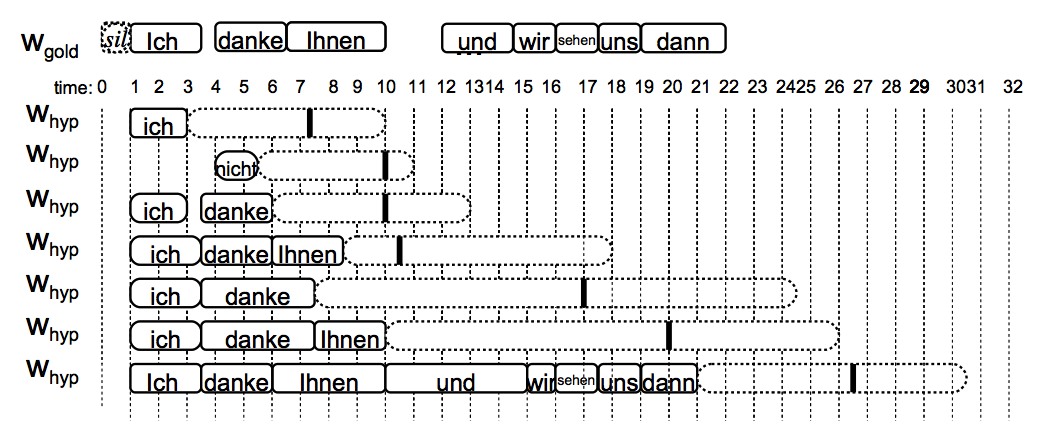
\includegraphics[width=1.0\textwidth]{images/gsphal.png}
 \caption{Google+Sphinx output with improved timing. Vertical lines show
 the time, by which Google was ready with the corresponding hypothesis.
 Right borders of the dotted boxes show at what point of time Sphinx was ready
 with its alignment.}
  \label{fig:conf_al_timing}
\end {figure}

Comparison of visualization results with the corresponding Google
output (\ref{fig:google_ouput}) demonstrates qualitative timing improvement in terms
alignment quality, whereas the WER remains unchanged, as the output contains
the same final result as that of Google alone. The number of hypotheses is
smaller, because Sphinx gets incremental results for processing only when
forced alignment of one result is finished.  If during Sphinx processing time
Google produce additional hypotheses, these hypotheses are skipped and only the
last one is taken for new processing. 

However, an obvious disadvantage of this alignment approach is additional
latency produced by Sphinx during alignment.
Alignment task, where the search path is known and defined is less time
consuming as recognizing, demands nevertheless computation time.  Computation
time depends on the processing power. If the Sphinx processing time could have
been neglected, than we get an model of Google+Sphinx recognizer,
comparable to Google in WERs and having an improved timing.

\subsection {Alignment + Recognition Mode  of the Google+Sphinx Recognizer}

In the second approach Sphinx returns not only alignment result, based on Google
ASR, but continues with recognition, while waiting for the new Google incremental result. 
This approach solves several tasks. First, we should get more precise alignment 
in case of excessive input stream. Moreover, excessive input stream is
even desirable as only additional frames guarantees recognition start after
alignment is finished. Second, Sphinx produces some results with better
timeliness, if it has finished alignment and is waiting for new Google
hypotheses. Third, it possible to use the Google result to manipulate the search
path in search graph of Sphinx and theoretically change to a path proposed by
Google, if this path exist. 

\begin{figure}[htbp]
  \centering 
 
 \lstdefinestyle{nonumbers} 
{numbers=none}  
\lstset{language=XML}  
%\begin{lstlisting}[frame=single]
 %backgroundcolor=\color{white}, 
 %\begin{lstlisting}  
\begin{lstlisting}[frame=single]]
...
      <component name="linguistFA"type=
      "edu.cmu.sphinx.linguist.dflat.DynamicFlatLinguist"> 
      <property name="logMath" value="logMath"/>
        <property name="grammar" value="ngramGrammar"/> 
        <!--  <property name="grammar" value=
        "myjsgfGrammar"/>--> 
        <property name="acousticModel" value=
        "acousticModel"/>
        <property name="wordInsertionProbability" value=
        "${wordInsertionProbability}"/>
        <property name="silenceInsertionProbability" value=
        "${silenceInsertionProbability}"/>
        <property name="languageWeight" value=
        "${languageWeight}"/>
        <property name="unitManager" value="unitManager"/>
    </component>
...
\end{lstlisting} 
 \caption{An extract from the configuration file for Google+Sphinx Recognizer in
 alignment and recognition mode.}
  \label{fig:conf_al_rec}
\end {figure}


Configuration of Google+Sphinx recognizer in alignment and recognition mode
uses dynamic flat linguist, because of the  advantages, described in the chapter
\ref{ch:sphinx}. As grammars the following types were tested: JSGF grammar
and n-gram grammar.  However, by contrast with
standard grammars in Sphinx these grammars are combined with alignment grammar 
in their implementation. Example configuration of the linguist is shown in the
figure  \ref{fig:conf_al_rec}.


As language models two types of language models were
available. The first one is  verbmobil language model, generated from the
selected number of texts from verbmobil domain with  4604 1-grams,  38548
2-grams and 80671 3-grams. The second one is a simplified language model, generated
only from the transcriptions, contained in the test data with 146 1-grams,
248 2-grams and 342 3-grams. The simplified language model is also runnable in
combination with flat linguist. Whereas  with the flat linguist and the bigger language model the 
application runs out of memory. 

The grammars are combined in the following way. The first node is
a starting node. After the starting node there is a path, consisting of nodes,
built from a set text (see figure  \ref{fig:graph}). The last alignment
node is connected to multiple paths in the second part of the graph, build from n-gram
or JSGF grammar. The last node of the graph is the end node.
\begin{figure}[htbp]
  \centering
    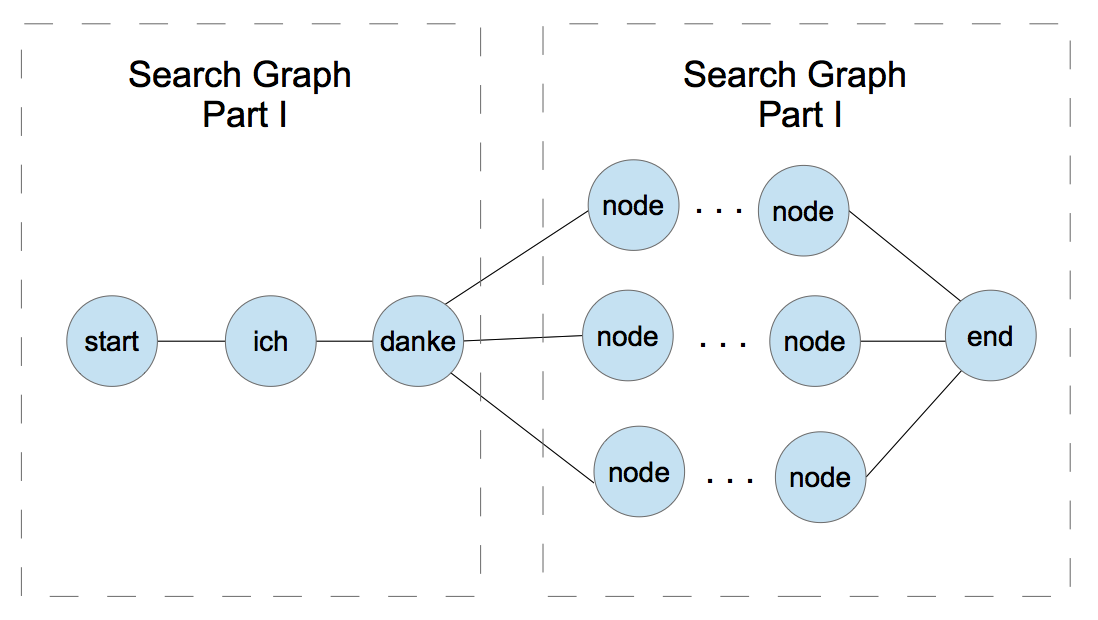
\includegraphics[width=1.0\textwidth]{images/searchgraph.png}
 \caption{Schematic representation of the search graph of Google+Sphinx
 recognizer in combined mode. In the example the text set for alignment is
 \textit {ich danke}.}
  \label{fig:graph}
\end {figure}

\subsection {Alignment + Recognition with JSGF Grammar}
To demonstrate that alignment and recognition are able to be combined any
type of JSGF grammar can be used. However, as JSGF grammar describe 
relative small command languages, we used a phone loop grammar in JSGF format,
suitable for more universal tasks.

An example of such grammar is shown in the figure   \ref{fig:phone_loop}

\begin{figure}[htbp]
\lstset{language=XML} 
 % \centering 
%  \lstset{
%   literate={@}{{\"u}}1
% }
%  \lstdefinestyle{nonumbers} 
%  {numbers=none} 
%  
%  
% %\begin{center}
\begin{lstlisting}[frame=single]
grammar phones;

public <phones> = (2: | 6 | 9 | @ | C | E | E: | I | N | O |
OY | Q |S | SIL | U | Y | Z  | a | a: | aI | aU | b | d |
e |  e: | f | g |h | i | i: |j | k | l | m | n | o | o: |
p| r | s |  t | u | u: | v | x | y: | z)*;
\end{lstlisting}
 \caption{An extract from the dictionary file.}
  \label{fig:phone_loop}
\end {figure}

Described phone-loop grammar is prototypical and uses no weights. Result of the
recognition of audio with transcription \textit {ich danke ignen und wir sehen
uns dann}, using the phone-loop grammar   \ref{fig:phone_loop} are shown in the
figure \ref{fig:phone_loop_res}.
\begin{figure}[htbp]
 \centering 
\begin{center}
\begin{lstlisting}[frame=single]
0.000	0.110	<sil>
0.110	0.340	ich
0.340	0.610	danke
0.610	1.050	ihnen
1.050	1.190	<sil>
1.190	1.230	r
1.230	1.290	o
1.290	1.400	o:
1.400	1.450	n
1.450	1.520	m
1.520	1.560	i
1.560	1.610	l
1.610	1.650	s
1.650	1.690	@
1.690	1.730	n
1.730	1.800	o
1.800	1.840	n
1.840	1.890	s
1.890	1.930	h
1.930	1.980	a
1.980	2.050	n
2.050	2.090	b
2.090	2.140	i
2.140	2.180	m
2.180	2.220	o
2.220	2.280	v
2.280	2.290	e
\end{lstlisting}
\end{center}
%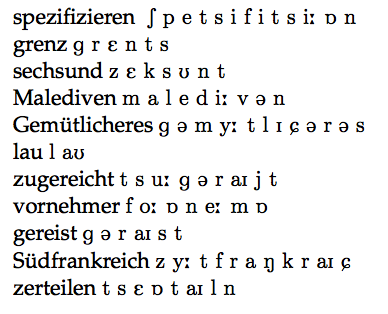
\includegraphics[width=0.5\textwidth]{images/dic.png}
 \caption{Alignment + Recognition result, using combined grammar, based on
 fixed input ``ich danke ihnen'' and phone-loop JSGF grammar for the audio,
 having transcription ``ich danke ihnen und wir sehen uns dann''
 (\ref{fig:phone_loop_res}).}
  \label{fig:phone_loop_res}
\end {figure}
Combination of alignment grammar with phone-loop JSGF grammar shows, that it is
possible to get some faster results from Sphinx, after the Google path is
already finished. At the moment the new result from Google is not yet
considered, because it is either not there due to latency or because the
processing of the audio is still running. 
%An example of the output, using such a
%grammar is shown in the picture \ref {fig: to do}. 

%\ldots here also some comments to the picture above

However, an obvious disadvantage of the above described approach that it is not 
possible to get use of the already recognized result, produced by Google as two
grammars (alignment and JSGF) are practically independent from each other.
Google produce always finished words or phrases as incremental output, followed
by silence. If the Google hypotheses were unfinished words it would be possible
to look in the JSGF Grammar for the most possible words endings. In our case
however, the only way to improve the recognition quality in the combination is
to improve the quality of phone-loop grammar output. For future there should be considered a
possibility to develop a more sophisticated grammar, based on phones
frequency and alternation rules generally in the language and in the selected
vocabulary in particular. 
\subsection {Alignment + Recognition with N-Gram Grammar}
The second approach to the combination of Google+Sphinx in alignment
and recognition mode presupposes the use of the implemented mixed grammar, based
on standard alignment and n-gram grammar of CMU Sphinx.  The search graph built
from this grammar looks as depicted in the figure \ref{fig:graph}, whereas the
first part of the graph is build from the set text string and the second part of
the graph is created on the basis of the n-gram grammar, loaded from the default
language model. 

In the first case, when in the second part of the graph there is no path,
proposed by Google, the last node of first part of the graph is connected with the
starting node in the second search graph. In the second case, when there is a
path, proposed by Google, the last node in the first part of the graph  is
deleted and second last node is connected to the a branch node in the second
part of the graph, that equals to the deleted last node in the first part of
the graph. 

In the present implementation when new text string is set  the
condition is checked if the whole path, proposed by the Google hypotheses exists in the second part of the
graph, build from n-gram grammar. For  example, if the set text equals \textit
{ich danke} the next node could be the first node of the whole second graph or the node 
\text {ich} is connected to the node \textit {danke} in the second search graph.
Additionally the existence of the whole path  \textit
{ich danke} in the graph is checked. 

Result of the recognition of audio with transcription \textit {ich danke ihnen
und wir sehen uns dann}, using n-gram grammar   is shown in
the figure  \ref{fig:ngram_res}.

\begin{figure}[htbp]
 \centering 
\begin{center}
\begin{lstlisting}[frame=single]
0.000	0.110	<sil>
0.110	0.300	ich
0.300	0.400	sage
0.400	0.610	danke
0.610	1.020	ihnen
1.020	1.470	und
1.470	1.590	wir
1.590	1.750	sehen
1.750	1.880	uns
1.880	2.290	dann>
\end{lstlisting}
\end{center}
%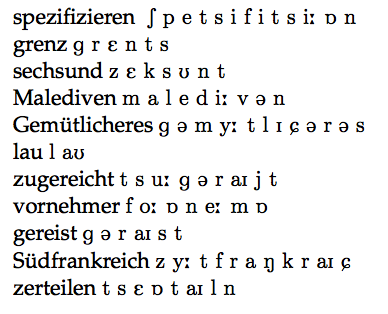
\includegraphics[width=0.5\textwidth]{images/dic.png}
 \caption{Alignment + Recognition result, using combined grammar, based on
 fixed input ``ich sage danke'' and n-gram grammar and simplified language
 model for the audio, having transcription ``ich danke ihnen und wir sehen uns
 dann'' (\ref{fig:phone_loop_res}).}
  \label{fig:ngram_res}
\end {figure}















%\section {forced alignment mode versus }





% The initialisation and implementation of the SearchGraph is realised by
% Sphinx-4. The choice and alternation of the path in
% the SearchGraph depends on the Google incremental hypotheses. 
% When the new Google hypotheses differs from the present hypotheses in the
% SearchGraph, the SearchGraph is reseted and the hypotheses path is
% corrected.  Timeliness improvement is supposed to be achieved by faster results
% produced by Sphinx, whereas the path in the Sphinx SearchGraph is predetermined
% by Google incremental result. The last means that we get the same final results
% for Google and Google + Sphinx, but timeliness of Google + Sphinx
%is expected to be improved. 
